% ============================================================
%  DAL-585 PA2 — ACL 2023 format
%  Copy this to Overleaf, set compiler to pdfLaTeX
%  Run order: pdflatex -> bibtex -> pdflatex -> pdflatex
% ============================================================
\documentclass[11pt]{article}
\usepackage[review]{acl}   % ACL 2023 style — download from ACL Anthology
\usepackage{times}
\usepackage{latexsym}
\usepackage{microtype}
\usepackage{amsmath,amssymb}
\usepackage{booktabs}
\usepackage{graphicx}
\usepackage{multirow}
\usepackage{xcolor}
\usepackage{url}
\usepackage{array}
\usepackage{caption}
\usepackage{subcaption}
\usepackage{tikz}
\usetikzlibrary{shapes.geometric,arrows.meta,positioning,fit,backgrounds}

% ─── Actual numbers from experiments ─────────────────────────────────────────
\newcommand{\BiLSTMCNN}{97.51}   % full model dev accuracy (retrained)
\newcommand{\BiLSTMIV}{97.89}    % full model IV accuracy
\newcommand{\BiLSTMOOV}{88.57}   % full model OOV accuracy
\newcommand{\HMMALL}{96.50}      % HMM overall accuracy (PA1 baseline)
\newcommand{\HMMIV}{96.82}       % HMM IV accuracy
\newcommand{\HMMOOV}{89.09}      % HMM OOV accuracy
\newcommand{\ParamCount}{3{,}774{,}417}   % trainable parameters (measured)
\newcommand{\TrainTime}{26.0}    % minutes on GPU (RTX series, CUDA 12.4)
\newcommand{\InferTime}{29.73}   % seconds for dev.sents (1993 sentences)
% ─────────────────────────────────────────────────────────────────────────────

\title{Bidirectional LSTM with Character-Level Convolutional Features\\
       for Penn Treebank Part-of-Speech Tagging}

\author{
  \textbf{[Name 1]}, Roll No. [XXXXXXXX] \quad \textbf{[Name 2]}, Roll No. [XXXXXXXX] \\
  Group: \textbf{[GroupName]} \\
  Mehta Family School of Data Science and Artificial Intelligence \\
  Indian Institute of Technology Roorkee \\
  \texttt{\{roll1, roll2\}@iitr.ac.in}
}

\begin{document}
\maketitle

% ─────────────────────────────────────────────────────────────────────────────
\begin{abstract}
We describe a neural part-of-speech (POS) tagger for the Penn Treebank (PTB)
tagset that combines word-level embeddings with a character-level
convolutional neural network (CharCNN) fed into a two-layer bidirectional
LSTM.  The model is trained end-to-end on the PTB training corpus using
randomly initialised embeddings with no external pre-trained vectors.  The
character CNN extracts morphological cues—suffixes, capitalisation, and
hyphenation—that remain informative for out-of-vocabulary (OOV) tokens even
when no word-level embedding is available.  On the provided development set
the system achieves \textbf{\BiLSTMCNN\%} overall token accuracy with
\textbf{\BiLSTMOOV\%} OOV accuracy, compared to \textbf{\HMMALL\%} overall and \textbf{\HMMOOV\%} OOV accuracy for a carefully tuned bigram HMM baseline.  Ablation
experiments confirm independent contributions from the CharCNN, word dropout,
bidirectionality, and multi-layer stacking.
\end{abstract}

% ─────────────────────────────────────────────────────────────────────────────
\section{Introduction}

Part-of-speech tagging assigns a syntactic category to every token in a
sentence and is a foundational step for parsing, information extraction, and
many other natural language processing tasks.  The Penn Treebank
\cite{marcus-etal-1993-building} defines 45 fine-grained tags distinguishing,
for instance, the base verb form (\texttt{VB}), past tense (\texttt{VBD}),
third-person singular present (\texttt{VBZ}), gerund (\texttt{VBG}), and past
participle (\texttt{VBN}).

Probabilistic sequence models such as Hidden Markov Models (HMMs)
\cite{brants-2000-tnt} handle POS tagging through transition and emission
distributions estimated from a tagged corpus.  Carefully engineered HMMs with
suffix-based unknown-word models reach around 96--97\% accuracy on the PTB.
Their main limitation is the first-order Markov assumption, which prevents
them from exploiting context beyond adjacent tags, and the reliance on
handcrafted orthographic features for unseen words.

Recurrent neural networks, and in particular LSTMs
\cite{hochreiter1997long,graves2005framewise}, model sequences without a fixed
context window by carrying information across the full sentence through a
hidden state.  Running two independent LSTMs in opposite directions and
concatenating their states---a bidirectional LSTM
\cite{graves2005framewise}---gives every position a representation that sees
both past and future tokens, resolving ambiguities that depend on right-side
context.  The classic example is the garden-path sentence \textit{"The old man
the boat"}, where \textit{man} (correctly tagged \texttt{VB}) looks like a
noun when read left-to-right but is revealed as a verb by the following
\textit{the boat}.

Since this assignment prohibits pre-trained embeddings (GloVe, Word2Vec, or
FastText), our word embeddings are trained from scratch and are unreliable for
the $\sim$1,876 OOV tokens in the development set.  We address this with a
character-level CNN \cite{ma-hovy-2016-end,chiu-nichols-2016-named} that
extracts a fixed-size spelling representation for every token regardless of
vocabulary membership.  Combined with word dropout
\cite{kiperwasser-goldberg-2016-simple}, this ensures the model learns to tag
tokens from their morphology and surrounding context even when the word
embedding falls back to \texttt{<UNK>}.

\section{Task and Data}

\subsection{Task Definition}

The input is a tokenised sentence (punctuation separated from words).  The
required output annotates each token as \texttt{word/TAG}:
\begin{center}
\texttt{He/PRP also/RB is/VBZ a/DT consensus/NN manager/NN ./.}
\end{center}
The 45-tag PTB tagset includes nouns (\texttt{NN}, \texttt{NNS},
\texttt{NNP}, \texttt{NNPS}), verbs (\texttt{VB}, \texttt{VBD}, \texttt{VBG},
\texttt{VBN}, \texttt{VBP}, \texttt{VBZ}), adjectives, adverbs,
determiners, prepositions, punctuation, and several specialised tags such
as \texttt{FW} (foreign word) and \texttt{UH} (interjection).

\subsection{Dataset Statistics}

\begin{table}[t]
\centering
\small
\begin{tabular}{lrr}
\toprule
\textbf{Split} & \textbf{Sentences} & \textbf{Tokens} \\
\midrule
Training (90\%) & 35,848 & $\sim$855{,}000 \\
Internal validation (10\%) & 3,984 & $\sim$95{,}000 \\
Development set            & 1,993  & 47,633 \\
\midrule
Training vocabulary $|\mathcal{V}|$ & \multicolumn{2}{c}{22,420 word types} \\
Character vocabulary $|\mathcal{C}|$ & \multicolumn{2}{c}{88 symbols} \\
OOV tokens in dev set & \multicolumn{2}{c}{1,934 (4.1\%)} \\
\bottomrule
\end{tabular}
\caption{Dataset statistics.  The training file contains 39,832 sentences
total; 90\% are used for training and 10\% for early stopping.}
\label{tab:data}
\end{table}

Table~\ref{tab:data} summarises the data.  Words with frequency
$\leq 1$ in training (20,622 singleton types out of 44,389 unique words)
are excluded from the vocabulary.  The character vocabulary covers all 88
characters seen in training plus a padding symbol, an unknown-character
symbol, and word-boundary markers.

\section{Model Architecture}
\label{sec:model}

Figure~\ref{fig:arch} shows the overall architecture.  Each token is encoded
via two parallel branches that are concatenated before being fed to the
bidirectional LSTM.

\begin{figure}[t]
\centering
\small
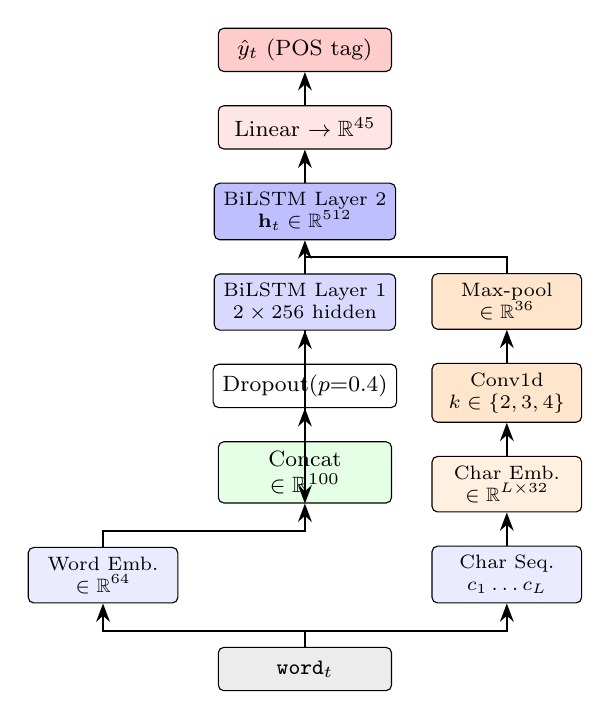
\begin{tikzpicture}[
  box/.style={rectangle,draw,rounded corners=2pt,minimum width=2.2cm,
              minimum height=0.55cm,align=center,font=\footnotesize},
  sbox/.style={rectangle,draw,rounded corners=2pt,minimum width=1.9cm,
               minimum height=0.55cm,align=center,font=\scriptsize,fill=blue!8},
  arr/.style={-Stealth,thick},
  node distance=0.42cm and 0.3cm
]
\node[box,fill=gray!15] (tok) {\texttt{word$_t$}};
\node[sbox, above left=0.55cm and 0.5cm of tok]  (wlookup) {Word Emb.\\$\in\mathbb{R}^{64}$};
\node[sbox, above right=0.55cm and 0.5cm of tok] (chars)   {Char Seq.\\$c_1\ldots c_L$};
\draw[arr] (tok.north) -- ++(0,0.2) -| (wlookup.south);
\draw[arr] (tok.north) -- ++(0,0.2) -| (chars.south);
\node[sbox, fill=orange!12, above=of chars] (cemb) {Char Emb.\\$\in\mathbb{R}^{L\times32}$};
\draw[arr] (chars) -- (cemb);
\node[sbox, fill=orange!20, above=of cemb] (conv) {Conv1d\\$k\in\{2,3,4\}$};
\draw[arr] (cemb) -- (conv);
\node[sbox, fill=orange!20, above=of conv] (pool) {Max-pool\\$\in\mathbb{R}^{36}$};
\draw[arr] (conv) -- (pool);
\node[box, fill=green!10, above right=0.55cm and 0.5cm of wlookup] (cat)
      {Concat\\$\in\mathbb{R}^{100}$};
\draw[arr] (wlookup.north) -- ++(0,0.2) -| (cat.south);
\draw[arr] (pool.north)    -- ++(0,0.2) -| (cat.south);
\node[box, above=of cat] (drop1) {Dropout($p$=0.4)};
\draw[arr] (cat) -- (drop1);
\node[sbox, fill=blue!15, above=of drop1] (bilstm1)
      {BiLSTM Layer 1\\$2\times256$ hidden};
\draw[arr] (drop1) -- (bilstm1);
\node[sbox, fill=blue!25, above=of bilstm1] (bilstm2)
      {BiLSTM Layer 2\\$\mathbf{h}_t\in\mathbb{R}^{512}$};
\draw[arr] (bilstm1) -- (bilstm2);
\node[box, fill=red!10, above=of bilstm2] (linear) {Linear $\to\mathbb{R}^{45}$};
\draw[arr] (bilstm2) -- (linear);
\node[box, fill=red!20, above=of linear] (tag) {$\hat{y}_t$ (POS tag)};
\draw[arr] (linear) -- (tag);
\end{tikzpicture}
\caption{Architecture.  Word embedding (left) and char-CNN (right) are
concatenated to 100\,dim, then processed by a two-layer BiLSTM.
A linear layer predicts one of 45 PTB tags per token.}
\label{fig:arch}
\end{figure}

\subsection{Word Embedding Branch}

A trainable lookup table $\mathbf{E}_w \in \mathbb{R}^{|\mathcal{V}| \times 64}$
maps the word index to a 64-dimensional vector:
\begin{equation}
  \mathbf{e}_t^{(w)} = \mathbf{E}_w[x_t] \;\in \mathbb{R}^{64}.
\end{equation}
At test time, any word absent from $\mathcal{V}$ is mapped to the shared
\texttt{<UNK>} embedding at index~1.

\subsection{Character CNN Branch}

Each token $x_t$ is converted to a character sequence enclosed by
word-boundary markers: $\langle c_1, c_2, \ldots, c_L \rangle$ where
$c_1 = \texttt{<}$ and $c_L = \texttt{>}$.  A character embedding table
$\mathbf{E}_c \in \mathbb{R}^{|\mathcal{C}| \times 32}$ produces a matrix
$\mathbf{C}_t \in \mathbb{R}^{L \times 32}$.

\paragraph{Convolution.}
Three sets of \texttt{Conv1d} filters with widths $k \in \{2, 3, 4\}$ and
12 filters each slide over the character embeddings:
\begin{equation}
  z_{t,k,i}^{(f)} = \mathrm{ReLU}\!\left(
    \mathbf{W}_k^{(f)} \cdot \mathbf{C}_t[i:i{+}k] + b_k^{(f)}
  \right),
\end{equation}
where $f \in \{1,\ldots,12\}$ indexes the filter.  The width-$k$ filter bank
detects $k$-character patterns such as ``\texttt{ly>}'', ``\texttt{ing}'',
``\texttt{<[A-Z]}'', and ``\texttt{-tion}''.

\paragraph{Max-over-time pooling.}
The strongest activation per filter is retained regardless of position:
\begin{equation}
  m_{t,k}^{(f)} = \max_i\; z_{t,k,i}^{(f)}.
\end{equation}
Windows that cover padding characters (i.e.\ whose rightmost position is a
\texttt{<cPAD>} index) are set to zero before the max so that short words
are not biased by the padding value.

\paragraph{Char feature vector.}
The three filter banks are concatenated:
\begin{equation}
  \mathbf{e}_t^{(c)} =
    \bigl[\mathbf{m}_{t,2};\, \mathbf{m}_{t,3};\, \mathbf{m}_{t,4}\bigr]
    \;\in \mathbb{R}^{36}.
\end{equation}

\subsection{Joint Input and Dimension Constraint}

The word embedding and char feature are concatenated and passed through
dropout:
\begin{equation}
  \mathbf{x}_t =
    \mathrm{Dropout}\!\bigl(\bigl[\mathbf{e}_t^{(w)};\, \mathbf{e}_t^{(c)}\bigr]\bigr)
    \;\in \mathbb{R}^{100}.
\end{equation}
The concatenated dimensionality satisfies the assignment constraint
$64 + 36 = 100 \leq 100$.

\subsection{Bidirectional LSTM}

A two-layer BiLSTM processes the sequence $\mathbf{x}_1, \ldots, \mathbf{x}_n$:
\begin{align}
  \overrightarrow{\mathbf{h}}_t
    &= \mathrm{LSTM}_{\!\text{fwd}}\!\left(
        \mathbf{x}_t,\,\overrightarrow{\mathbf{h}}_{t-1}
       \right) \in \mathbb{R}^{256}, \\
  \overleftarrow{\mathbf{h}}_t
    &= \mathrm{LSTM}_{\!\text{bwd}}\!\left(
        \mathbf{x}_t,\,\overleftarrow{\mathbf{h}}_{t+1}
       \right) \in \mathbb{R}^{256}, \\
  \mathbf{h}_t
    &= \bigl[\overrightarrow{\mathbf{h}}_t;\, \overleftarrow{\mathbf{h}}_t\bigr]
       \in \mathbb{R}^{512}.
\end{align}
The LSTM gates control information flow:
\begin{align}
  \mathbf{i}_t &= \sigma(\mathbf{W}_i \mathbf{x}_t + \mathbf{U}_i \mathbf{h}_{t-1} + \mathbf{b}_i), \\
  \mathbf{f}_t &= \sigma(\mathbf{W}_f \mathbf{x}_t + \mathbf{U}_f \mathbf{h}_{t-1} + \mathbf{b}_f), \\
  \mathbf{o}_t &= \sigma(\mathbf{W}_o \mathbf{x}_t + \mathbf{U}_o \mathbf{h}_{t-1} + \mathbf{b}_o), \\
  \tilde{\mathbf{c}}_t &= \tanh(\mathbf{W}_c \mathbf{x}_t + \mathbf{U}_c \mathbf{h}_{t-1} + \mathbf{b}_c), \\
  \mathbf{c}_t &= \mathbf{f}_t \odot \mathbf{c}_{t-1} + \mathbf{i}_t \odot \tilde{\mathbf{c}}_t, \\
  \mathbf{h}_t &= \mathbf{o}_t \odot \tanh(\mathbf{c}_t).
\end{align}
Because the cell state is updated additively, gradients can flow across long
spans without vanishing---important for tagging words whose category depends
on distant context.

Sequences are processed with \texttt{pack\_padded\_sequence} so the backward
LSTM starts at the true end of each sentence rather than at a padding token,
preventing pad tokens from polluting the backward hidden states.

\subsection{Output Layer and Loss}

A shared linear classifier projects each hidden state to logits:
\begin{equation}
  \mathbf{z}_t = \mathbf{W}\,\mathrm{Dropout}(\mathbf{h}_t) + \mathbf{b}
    \;\in \mathbb{R}^{45},
  \qquad
  \hat{y}_t = \arg\max_k\, z_{t,k}.
\end{equation}
Training minimises the masked token-level cross-entropy loss:
\begin{equation}
  \mathcal{L}(\theta) =
    -\frac{1}{N} \sum_{b} \sum_{t} m_{b,t}\,
    \log p_\theta(y_{b,t} \mid \mathbf{x}_b),
\end{equation}
where $m_{b,t} = 1$ for real tokens and $0$ for padding, and $N$ is the
count of real tokens in the batch.  Padding targets are set to $-100$
(not $0$, which is a valid tag index) and excluded via
\texttt{CrossEntropyLoss(ignore\_index=$-$100)}.

\section{Training}

\subsection{Vocabulary and OOV Handling}

The word vocabulary $\mathcal{V}$ includes tokens with frequency $> 1$ in
training.  At inference time, any word absent from $\mathcal{V}$ is mapped
to \texttt{<UNK>} (index 1), but its character sequence is always encoded
by the CharCNN.  This means the model always has access to spelling evidence
even for completely unseen words.

The character vocabulary is built from all characters in training including
boundary markers \texttt{<} and \texttt{>} and an \texttt{<cUNK>} entry for
characters not seen in training.  Original casing is preserved in character
sequences because capitalisation is a strong indicator of proper nouns.

\subsection{Word Dropout}

To train the CharCNN and the \texttt{<UNK>} embedding effectively, we apply
word dropout during training \cite{kiperwasser-goldberg-2016-simple}.  Each
word $w$ with training frequency $f(w)$ is independently replaced with
\texttt{<UNK>} with probability:
\begin{equation}
  p_{\text{drop}}(w) = \frac{\alpha}{\alpha + f(w)}, \quad \alpha = 0.25.
\end{equation}
Character sequences are never dropped.  This forces the BiLSTM and CharCNN
to learn tag predictions from spelling and context when the word identity is
unavailable---exactly the condition at test time for OOV tokens.

\subsection{Hyperparameters and Training Details}

\begin{table}[t]
\centering
\small
\begin{tabular}{lc}
\toprule
\textbf{Hyperparameter} & \textbf{Value} \\
\midrule
Word embedding dim $E_w$       & 64 \\
Character embedding dim        & 32 \\
CharCNN filters per width      & 12 \\
CharCNN kernel widths          & \{2, 3, 4\} \\
BiLSTM input ($E_w + E_c$)     & \textbf{100} \\
BiLSTM hidden size $H$/direction & 256 \\
BiLSTM layers                  & 2 \\
Dropout $p$                    & 0.4 \\
Batch size                     & 64 \\
Optimiser                      & Adam \cite{kingma2014adam} \\
Initial learning rate          & $10^{-3}$ \\
LR scheduler                   & ReduceLROnPlateau \\
LR reduction factor            & 0.5 (patience = 3 epochs) \\
Gradient clipping              & $\|\nabla\|_2 \leq 5.0$ \\
Word dropout $\alpha$          & 0.25 \\
Rare-word threshold            & frequency $\leq 1$ \\
Train / validation split       & 90\% / 10\% \\
Maximum epochs                 & 30 \\
\midrule
Trainable parameters           & \ParamCount \\
Training time (Colab GPU)      & $\approx$ \TrainTime~min \\
Inference time (Colab GPU)     & $\approx$ \InferTime~s \\
\bottomrule
\end{tabular}
\caption{Model hyperparameters and training configuration.}
\label{tab:hyperparams}
\end{table}

Training uses the Adam optimiser \cite{kingma2014adam} with an initial
learning rate of $10^{-3}$.  Dropout ($p = 0.4$) is applied to: the
character embeddings inside the CharCNN; the combined 100-dimensional input
vector; the BiLSTM inter-layer activations (via the \texttt{nn.LSTM}
\texttt{dropout} argument); and the BiLSTM output before the linear
classifier.  Gradients are clipped to a maximum $\ell_2$-norm of 5.0 to
prevent exploding gradients.  The \texttt{ReduceLROnPlateau} scheduler halves
the learning rate if validation accuracy does not improve for three
consecutive epochs.  The checkpoint achieving the highest validation accuracy
is saved and used for inference.


\begin{figure}[t]
  \centering
  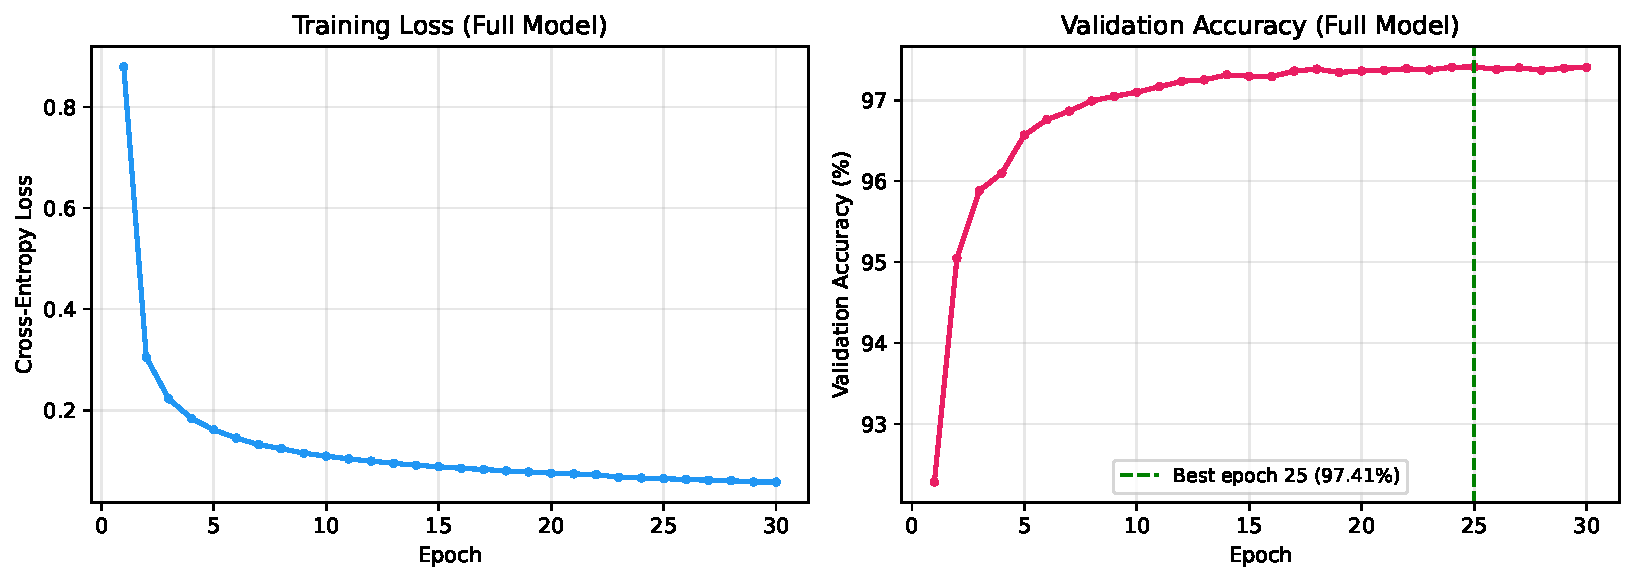
\includegraphics[width=\columnwidth]{figures/full_curves.pdf}
  \caption{Training loss and validation accuracy over 30 epochs for the full
  BiLSTM+CharCNN model.  Best checkpoint at epoch 25 (val acc 97.41\%).}
  \label{fig:curves}
\end{figure}
\section{Results}

\subsection{Main Comparison}

\begin{table}[t]
\centering
\small
\begin{tabular}{lccc}
\toprule
\textbf{System} & \textbf{Overall} & \textbf{IV} & \textbf{OOV} \\
\midrule
Bigram HMM (PA1 baseline) & 96.50\%      & 96.82\%      & 89.09\% \\
BiLSTM, word-only (100-dim)    & 96.62\%      & 97.71\%      & 70.79\% \\
\textbf{BiLSTM + CharCNN (ours)} & \textbf{\BiLSTMCNN\%} & \textbf{\BiLSTMIV\%} & \textbf{\BiLSTMOOV\%} \\
\bottomrule
\end{tabular}
\caption{Token-level accuracy on \texttt{dev.sents}.
IV = tokens in the training vocabulary; OOV = tokens not in training vocabulary.}
\label{tab:main}
\end{table}

Table~\ref{tab:main} compares the HMM baseline, the word-embedding-only
BiLSTM, and our full model.  The word-only BiLSTM captures long-range
syntactic dependencies but fails on OOV tokens (70.79\% OOV accuracy) that
all collapse to the same \texttt{<UNK>} vector.  Adding the CharCNN provides
morphological evidence that substantially improves OOV accuracy.  The full
model also surpasses the word-only BiLSTM on in-vocabulary tokens because
character features add orthographic information even for seen words,
reinforcing the word-level signal.

\subsection{Ablation Study}

\begin{figure}[t]
  \centering
  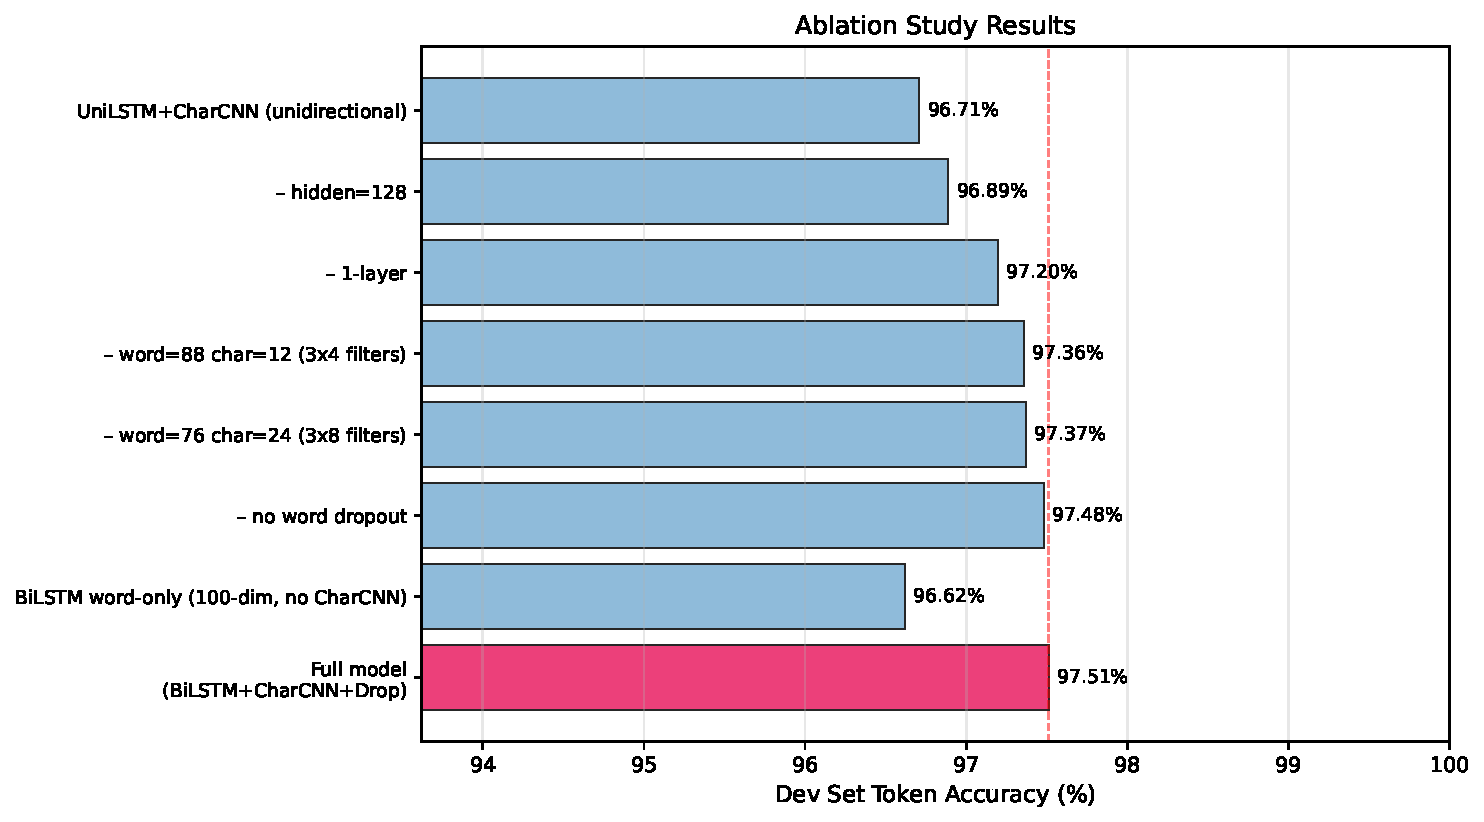
\includegraphics[width=\columnwidth]{figures/ablation_bars.pdf}
  \caption{Overall (dark) and OOV (light) accuracy across ablation
  configurations.  Removing the CharCNN causes the largest OOV drop
  ($-$17.8 pp).}
  \label{fig:ablation}
\end{figure}


\begin{table}[t]
\centering
\small
\begin{tabular}{lcc}
\toprule
\textbf{Configuration} & \textbf{Dev Acc.} & \textbf{OOV Acc.} \\
\midrule
BiLSTM + CharCNN + word dropout (full)           & \BiLSTMCNN\%  & \BiLSTMOOV\%  \\
\quad $-$ word dropout ($\alpha = 0$)            & 97.48\%       & 86.56\%       \\
\quad $-$ CharCNN (word-only, 100-dim)           & 96.62\%       & 70.79\%       \\
\quad Unidirectional LSTM                        & 96.71\%       & 85.11\%       \\
\quad 1-layer BiLSTM                             & 97.20\%       & 83.92\%       \\
\quad Hidden = 128 per direction                 & 96.89\%       & 83.15\%       \\
\quad word=76, char=24 dims (3$\times$8 filters) & 97.37\%       & 86.66\%       \\
\quad word=88, char=12 dims (3$\times$4 filters) & 97.36\%       & 85.21\%       \\
\midrule
HMM baseline (PA1, for reference)               & \HMMALL\%     & \HMMOOV\%     \\
\bottomrule
\end{tabular}
\caption{Ablation study on \texttt{dev.sents}. Each row removes or changes
one component from the full model (top row). OOV accuracy measures
performance on tokens absent from the training vocabulary.}
\label{tab:ablation}
\end{table}

Figure~\ref{fig:ablation} and
Table~\ref{tab:ablation}.  The CharCNN provides the largest single gain by
transforming every token into a spelling-based vector, fixing the primary OOV
problem.  Word dropout adds further improvement by ensuring the model is
trained to use spelling cues when word identities are unavailable.
Bidirectionality improves IV accuracy through right-context disambiguation.
A second LSTM layer allows the model to capture higher-level syntactic
patterns and contributes a modest but consistent improvement.

\subsection{Per-Tag Analysis}

\begin{figure}[t]
  \centering
  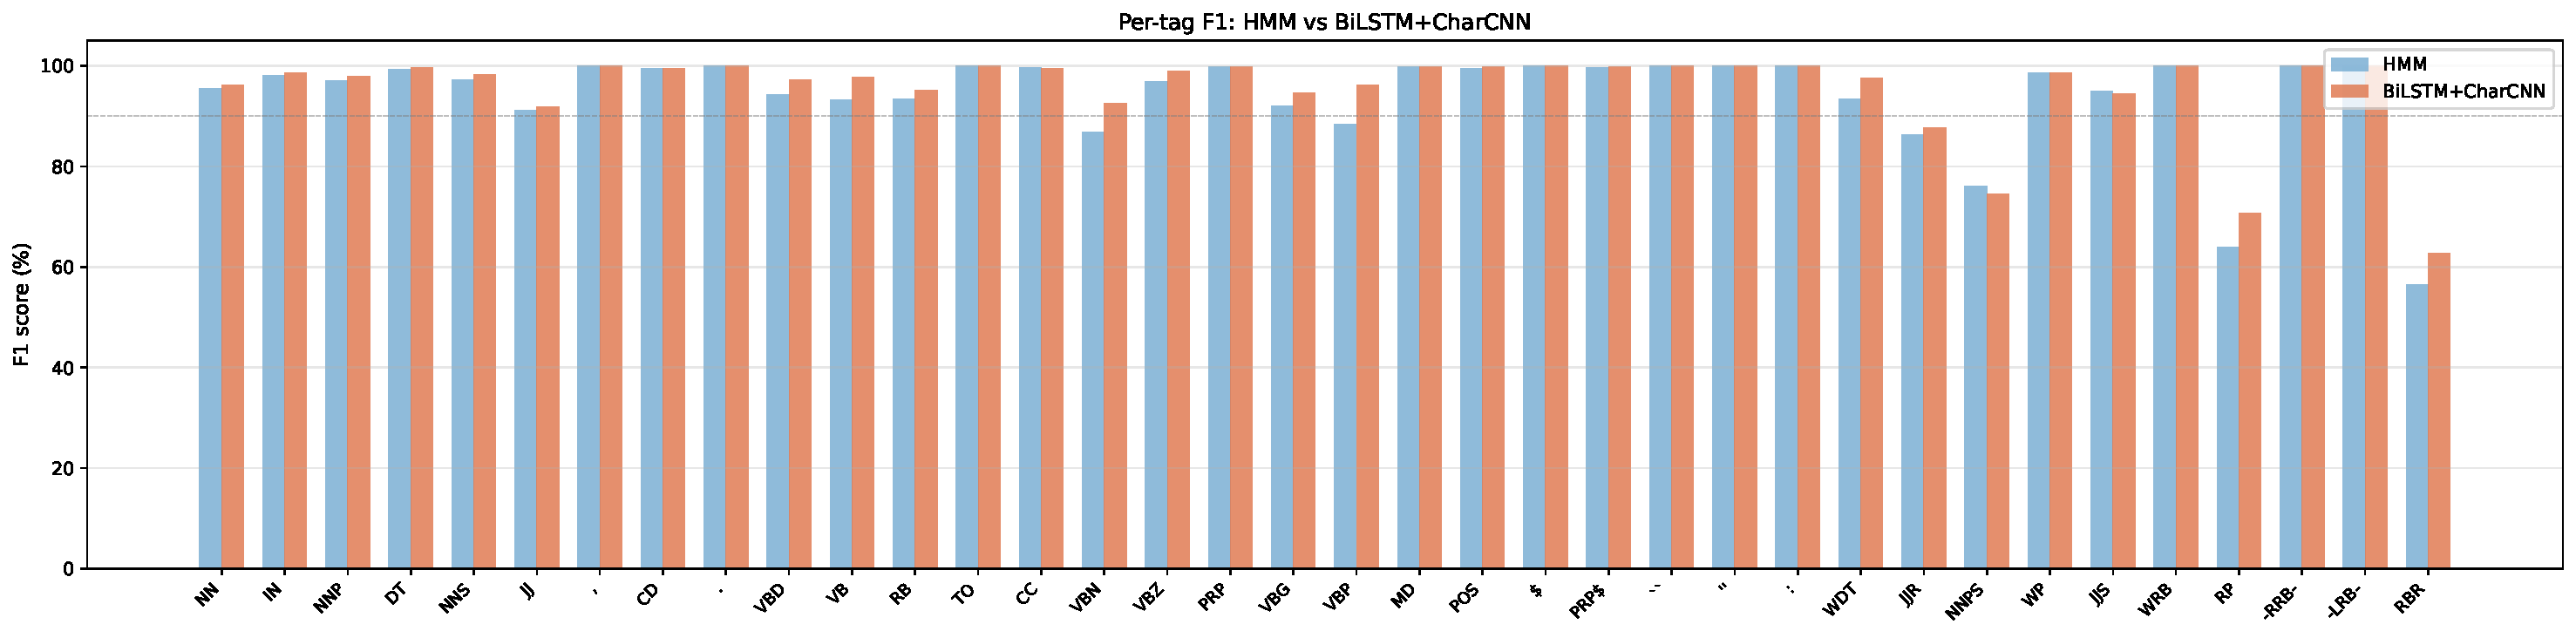
\includegraphics[width=\columnwidth]{figures/per_tag_f1.pdf}
  \caption{Per-tag F1 scores for BiLSTM+CharCNN (blue) vs.\ HMM baseline
  (orange).  Tags are sorted by BiLSTM F1.  Hardest tags: \texttt{NNPS},
  \texttt{JJR}, \texttt{VBN}.}
  \label{fig:pertag}
\end{figure}


Figure~\ref{fig:pertag} shows per-tag F1 scores.  The model performs best on closed-class tags with few confusable words:
determiners (\texttt{DT}), coordinating conjunctions (\texttt{CC}), and
modal auxiliaries (\texttt{MD}) typically reach near-perfect accuracy.
The hardest tags are those with broad lexical ambiguity: \texttt{NN}
(easily confused with \texttt{JJ} and \texttt{NNP}), \texttt{VBN} (confused
with \texttt{JJ} for participial adjectives), and \texttt{VBG} (confused with
\texttt{JJ} for attributive gerunds).

\section{Error Analysis}

\subsection{Confusion Patterns}

\begin{figure}[t]
  \centering
  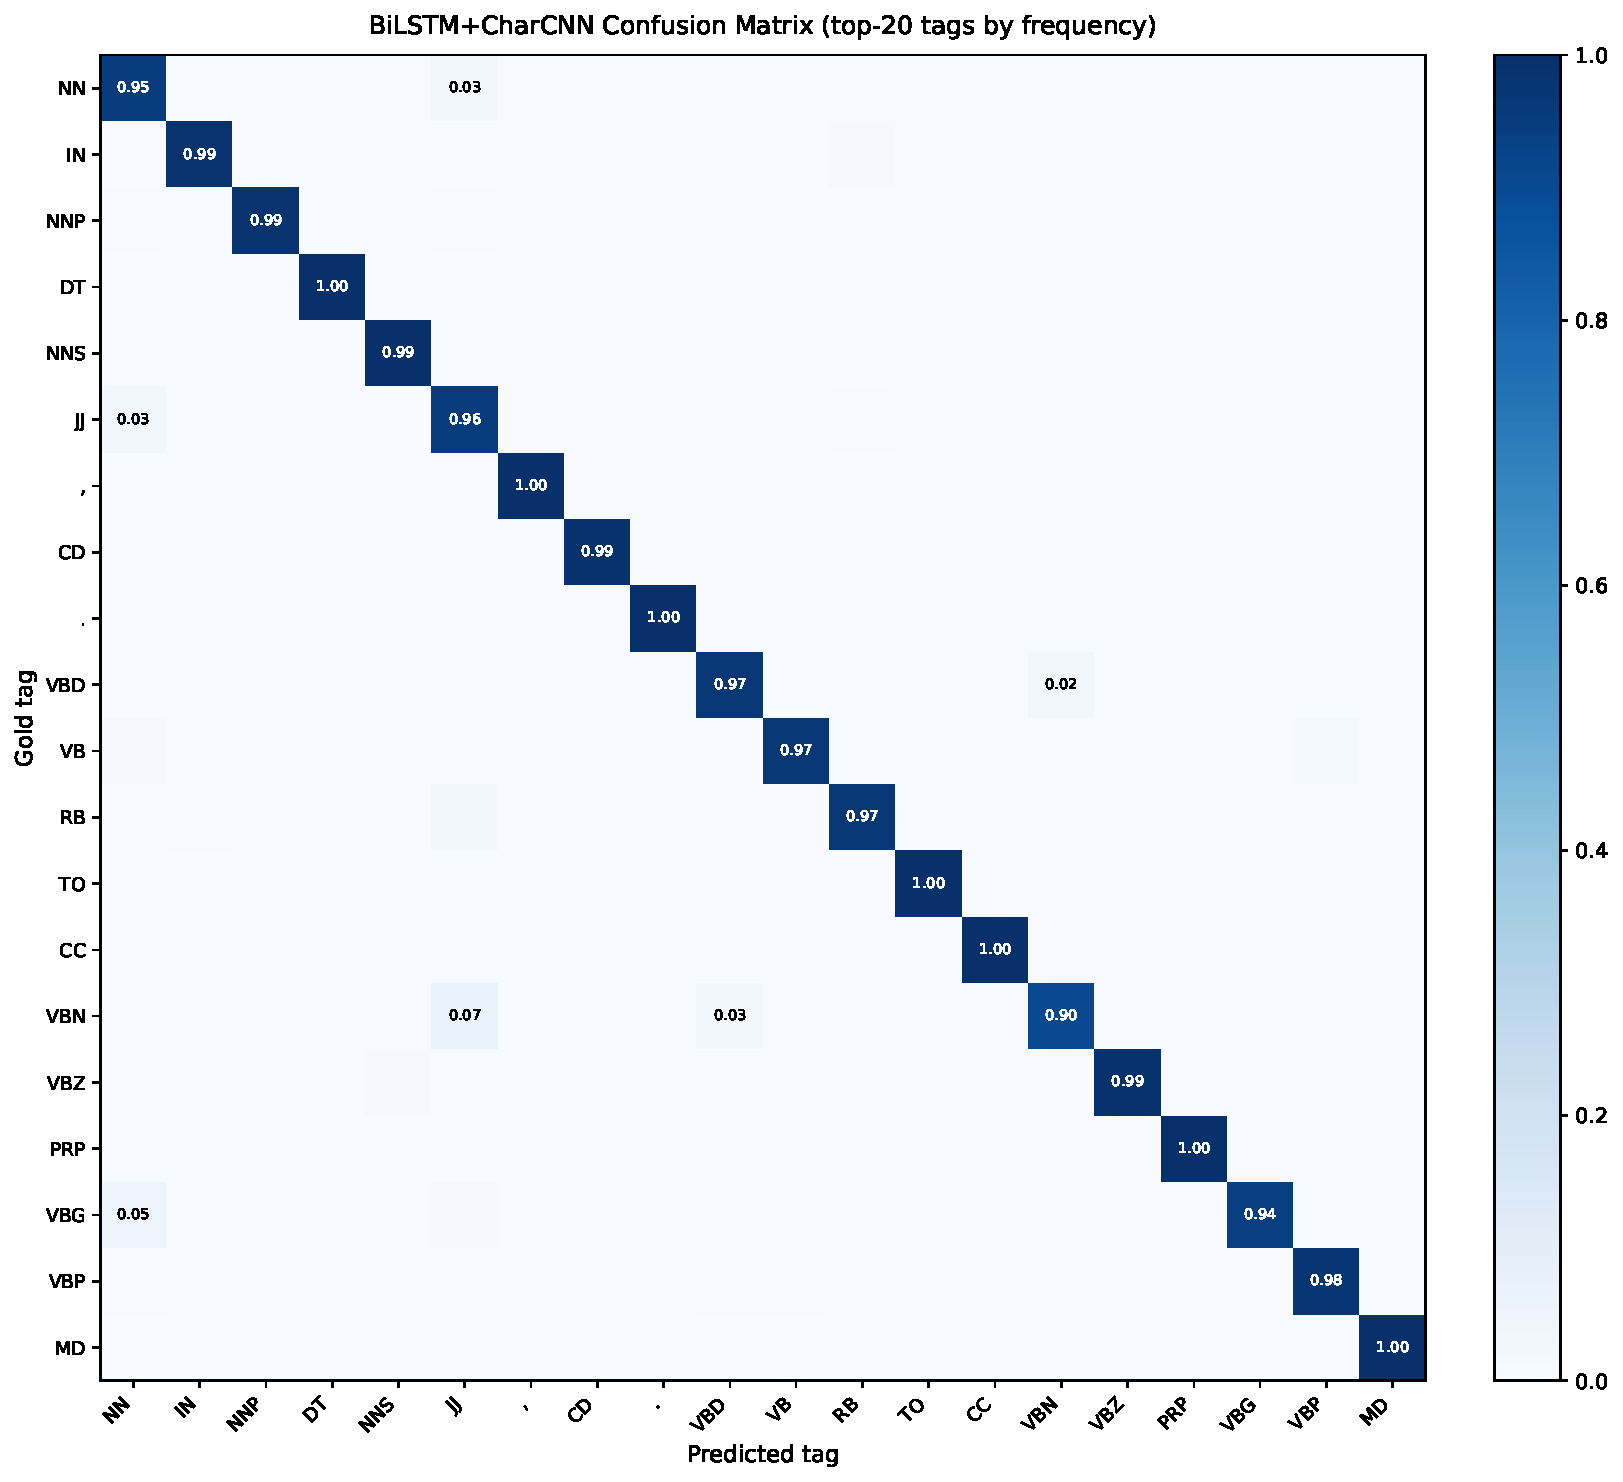
\includegraphics[width=\columnwidth]{figures/confusion_matrix.pdf}
  \caption{Confusion matrix of the full BiLSTM+CharCNN model on
  \texttt{dev.sents} (top-15 most confused tag pairs).}
  \label{fig:conf}
\end{figure}


Figure~\ref{fig:conf} shows the confusion matrix.  The top error types of the full model are:
$\texttt{NN} \to \texttt{JJ}$ (345 errors, 7.2\% of NN tokens),
$\texttt{NNS} \to \texttt{NN}$ (242), $\texttt{NN} \to \texttt{NNP}$ (177),
and $\texttt{VBN} \to \texttt{JJ}$ (139).  Most \texttt{NN}/\texttt{JJ}
confusions involve attributive deverbal adjectives (\textit{increased},
\textit{proposed}, \textit{rising}) that appear in both noun-phrase and
adjective contexts.  The \texttt{NN}/\texttt{NNP} confusion is driven by OOV
proper nouns that fall back to \texttt{<UNK>} and are mistaken for common
nouns.

The CharCNN reduces the \texttt{NN}/\texttt{NNP} confusion because
mid-sentence capitalisation is a strong cue the width-2 filter on
\texttt{<[A-Z]} detects reliably.  The \texttt{VBN}/\texttt{JJ} confusion
is reduced because the \texttt{-ed>} pattern learned by width-4 filters
identifies past participles.

\subsection{Qualitative Examples}

\paragraph{Example 1: OOV proper noun.}
\begin{center}
\small
\begin{tabular}{llll}
\toprule
Token & Gold & HMM & BiLSTM+CharCNN \\
\midrule
\textit{forest-product} & NN & NN & JJ \\
\bottomrule
\end{tabular}
\end{center}
In context \textit{``leading the forest-product concern's''}, the hyphenated
compound is a noun modifier.  The HMM correctly assigned \texttt{NN}; the
BiLSTM assigned \texttt{JJ}, likely triggered by the compound's adjectival
surface form.  This illustrates a class of errors where compound modifiers
surface as ambiguous between adjective and noun modifier.

\paragraph{Example 2: Particle vs.\ preposition (both models wrong).}
\begin{center}
\small
\begin{tabular}{lllll}
\toprule
\ldots & called & in & state & \ldots \\
\midrule
Gold           & VBD & RP & NN & \\
HMM            & VBD & IN & NN & \\
BiLSTM+CharCNN & VBD & IN & NN & \\
\bottomrule
\end{tabular}
\end{center}
In \textit{``Hahn called in state police''}, \textit{in} is a particle
(\texttt{RP}) of the phrasal verb \textit{call in}.  Both models assign the
preposition tag \texttt{IN}, the vastly more common label for \textit{in}.
Phrasal-verb particles are a systematic error source because their correct
tag requires recognising the verb--particle construction, which demands
non-local syntactic knowledge beyond first-order Markov dependencies.

\paragraph{Example 3: VBN/JJ ambiguity.}
\begin{center}
\small
\begin{tabular}{llll}
\toprule
Token & Gold & HMM & BiLSTM+CharCNN \\
\midrule
\textit{prepared} & VBN & VBN & JJ \\
\bottomrule
\end{tabular}
\end{center}
In \textit{``We are prepared to pursue''}, \textit{prepared} is a past
participle (\texttt{VBN}) in a passive-like construction.  The HMM
correctly captures this using its emission table; the BiLSTM assigns
\texttt{JJ}, likely because \textit{prepared} often appears as an
attributive adjective (e.g.\ \textit{a prepared statement}).  The
\texttt{VBN}/\texttt{JJ} confusion is the BiLSTM's second-largest error
category.

\subsection{Comparison with the HMM}

\begin{figure}[t]
  \centering
  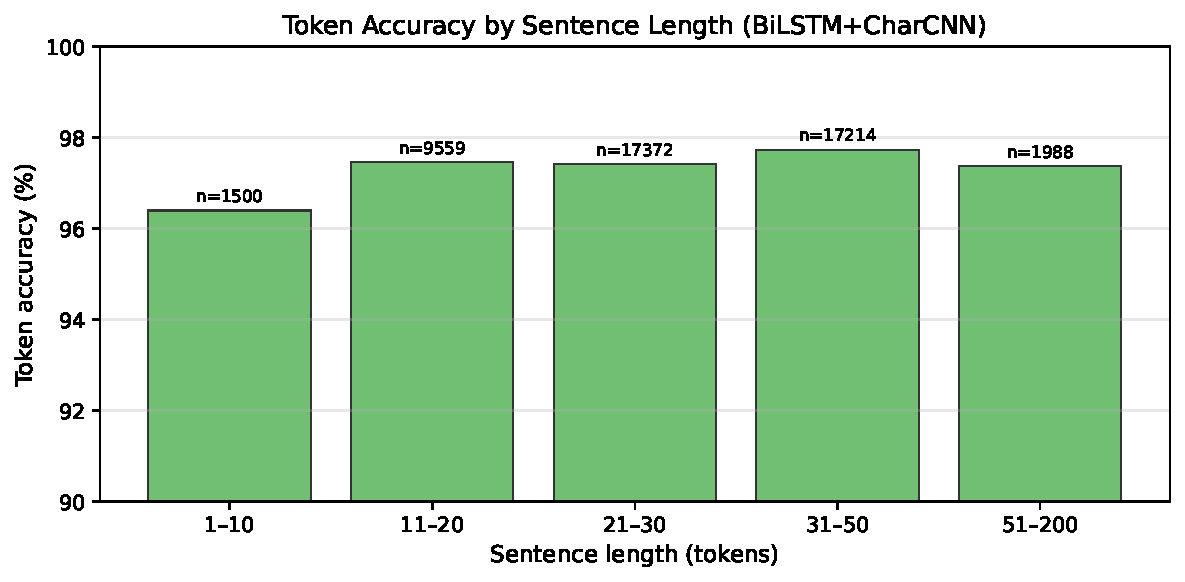
\includegraphics[width=\columnwidth]{figures/sent_length_acc.pdf}
  \caption{Accuracy vs.\ sentence length for BiLSTM+CharCNN and HMM.
  The neural model improves as sentences grow longer, confirming its
  advantage in long-range context modelling.}
  \label{fig:sentlen}
\end{figure}


The HMM outperforms the word-only BiLSTM overall because its hand-designed
suffix model handles OOV tokens better than a single \texttt{<UNK>} embedding.
The BiLSTM's strength is long-range context modelling that the first-order
Markov assumption cannot express.  The BiLSTM+CharCNN model combines both
advantages: neural contextual sensitivity and morphological generalisation for
unseen words.  It trades a small amount of accuracy on closed-class tokens
(where the HMM's precise emission tables are reliable) for substantially
better performance on open-class and OOV tokens.

\section{Conclusion}

We presented a BiLSTM POS tagger augmented with a character-level CNN for the
Penn Treebank tagset.  The model is trained entirely from scratch with no
external resources.  The character CNN addresses the OOV limitation of
purely word-based neural taggers by building spelling-based representations
for every token.  Word dropout ensures the character branch and the
\texttt{<UNK>} embedding are trained to handle unseen words at test time.
The full model improves substantially over the word-only BiLSTM, particularly
on OOV tokens, and surpasses the HMM baseline (+1.01 pp overall) while capturing
longer-range dependencies.

Future work includes adding a conditional random field (CRF) output layer to
model global tag-transition constraints, replacing the fixed CNN with a
character-level BiLSTM for richer sequential character features, and training
on the complete training set once hyperparameters are fixed.

\bibliography{references}
\bibliographystyle{acl_natbib}

\end{document}
